This walking example is presented to introduce \textit{bioptim}'s ability to deal with gait biomechanics as a multiphase problem with contact forces.
The goal was to estimate muscles activation by tracking markers trajectories, ground reaction forces and moments (Equations.~\ref{eq:ocp_markers}, ~\ref{eq:ocp_forces} and ~\ref{eq:ocp_moments}, respectively). 
The model was driven by muscle activation. 
To predict muscle activity, the objective function consisted in finding the least squared muscle activations $a_{i}$ (Equations.~\ref{eq:ocp_muscles}). 
Pure residual torques were also added to compensate potential underactuation from the model weaknesses and penalized as shown in equation ~\ref{eq:ocp_torques}.\\
The gait cycle was defined from the first heel strike to the end of the swing phase using a simplified 3D one-leg model with 12 DoFs and 17 muscles (pelvis + right lower limb). 
Based on experimental force plateform data and markers position, the stance was divided into three phases (heel, flatfoot and forefoot contacts) of fixed duration (0.05, 0.355 and 0.16s), to follow the natural rolling movement of the foot from heel strike to toe off.
The swing phase lasted 0.38 s. 
The interaction between the ground and the foot was modelled using a 4-contact points model located at the heel and the forefoot (first, fifth metatarsi and hallux).

The complete cycle was discretized in 90 intervals and the objective functions are written as follow :\\

%\[ 
%\resizebox{0.9\columnwidth}{!}{$ 
%\begin{aligned}
%\mathcal{J} = &\int_{t=0}^{T}\underbrace{\omega_1(\|m_p - m_m\|^{2})}_{\mathtt{TRACK\_MARKERS}}~ 
%+ ~ \underbrace{\omega_2(\|f_p - f_c\|^{2})}_{\mathtt{TRACK\_FORCES}}\\
%&+ ~ \underbrace{\omega_3(\|tau^f_p - tau^f_m\|^{2})}_{\mathtt{TRACK\_MOMENTS}}~
%\mathcal{J} = &\int_{t=0}^{T}\underbrace{\omega_1(\|m_p - m^*_m\|^{2})}_{\mathtt{TRACK\_MARKERS}}~ 
%+ ~ \underbrace{\omega_2(\|f_p - f^*_c\|^{2})}_{\mathtt{TRACK\_FORCES}}\\
%&+ ~ \underbrace{\omega_3(\|tau^f_p - tau^{f*}_m\|^{2})}_{\mathtt{TRACK\_MOMENTS}}~
%+ ~ \underbrace{\omega_4\|a\|^2}_{\mathtt{MIN\_ACTIVATION}}~dt, 
%\end{aligned}  
%$}  
%$}
%\addtag  
%\label{eq:ocp_walk}  
%\]

\begin{eqnarray}
\label{eq:ocp_markers}
\mathcal{J} = \sum_{i=1}^{N_i}\Bigg(\underbrace{\omega_1(\|m_p - m_m\|^{2})}_{\mathtt{TRACK\_MARKERS}}
\end{eqnarray}
\begin{eqnarray}
\label{eq:ocp_forces}
+ \underbrace{\omega_2(\|\sum_{c=1}^{N_c}F_p - F_m\|^{2})}_{\mathtt{TRACK\_FORCES}}
\end{eqnarray}
\begin{eqnarray}
\label{eq:ocp_moments}
+ \underbrace{\omega_3(\|\sum_{c=1}^{N_c}M_p - M_m\|^{2})}_{\mathtt{TRACK\_MOMENTS}}
\end{eqnarray}
\begin{eqnarray}
\label{eq:ocp_muscles}
+ \underbrace{\omega_4\int_0^T \sum_{i=1}^{N_i}~a_{i}^2~dt}_{\mathtt{MINIMIZE\_ ACTIVATION}})  
\end{eqnarray}
\begin{eqnarray}
\label{eq:ocp_torques}
+ \underbrace{\omega_5\int_0^T \sum_{i=1}^{2}~\tau_{i}^2~dt}_{\mathtt{MINIMIZE\_ TORQUE}}\bigg)
 \end{eqnarray}

where $\omega_{i}$ are the weighting factors ($\omega_1$=1e5, $\omega_2$=0.1, $\omega_3$=0.1, $\omega_4$=10, $\omega_5$=1), $T$ is the the duration, $N_i$ and $N_c$ are the number of time frames and contact points of the current phase. The indices $_p$ and $_m$ stand for predicted and measured data.\\

Non-slipping ($\mathtt{NON\_SLIPPING}$) and unilateral contact force ($\mathtt{CONTACT\_FORCE}$) constraints prevented the foot from slipping and pulling from the ground. 
In between phases, the use of the $\mathtt{IMPACT}$ state transition allowed to represent the gain or loss of contact(s) in the dynamics (e.g., swing phase to heel strike [thesis Felis - articles?]) \\

Fig.~\ref{fig:snapshots_multiphase_walking_cycle} shows the leg movements during the walking cycle. The mean tracking error on markers trajectories was 0.027 m (mean error on pelvic and foot markers was 0.0075 m and 0.0147 m, respectively). 
Concerning ground reaction forces tracking, the mean error was 4.85 N with an average $R^2$ at 0.9. 
Gluteal muscles were only activated during the stance phase and especially during the early flatfoot phase for the gluteus maximus with a maximal activation of 0.2. 
For the thigh muscles, the semimembranous, semitendinous and biceps femoris were activated during the early stance phase and terminal swing (maximal activation of 0.3, 0.4 and 0.4, respectively). 
The knee extensors, vastus lateralis, medialis and intermedius followed the same pattern and were mainly activated during the flatfoot phase. 
However, maximal activation of the rectus femoris appeared at early forefoot phase and early swing. Leg muscles were highly activated (saturation of gastocnemius lateralis and medialis) at the end of the stance and the early swing phase. 

\begin{figure*}[t!]
\centering
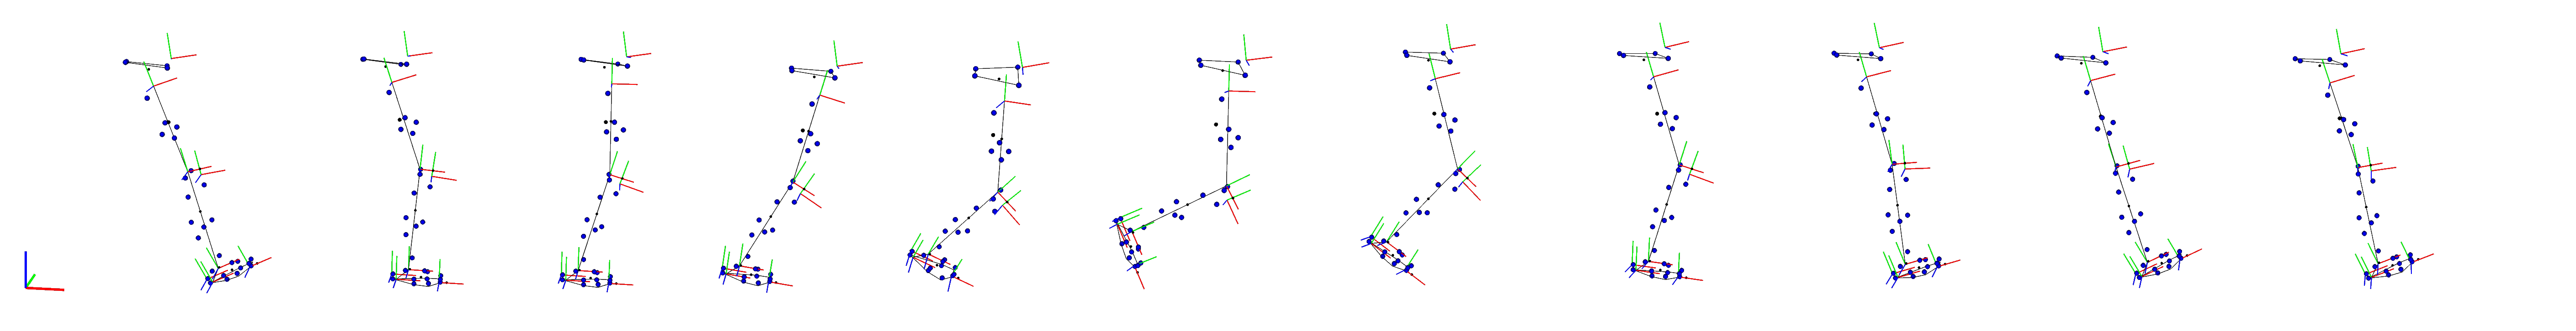
\includegraphics[width=\textwidth]{figures/multiphase_walking_cycle.png}\\
\caption{Snapshots of a walking gait cycle driven by muscles activation.}
\label{fig:snapshots_multiphase_walking_cycle}
\end{figure*}

%\begin{table}[h!]
%\caption{\small Objective terms of the Multiphase torque driven walking cycle }
%\label{tab:Multiphase_torque_driven_walking_cycle}
%\centering
%\begin{tabular}{c c c c}
%\toprule 
%& Type & Function & Weight \\ 
%\midrule
%$\#1$ & Lagrange & TRACK\_ STATE & $1e5$ \\ 
%\midrule
%$\#2$ & Lagrange & MINIMIZE\_ TORQUE\_ DERIVATIVE & $1e-2$ \\ 
%\midrule
%$\#3$ & Lagrange & TRACK\_ GRF & $1e-2$ \\ 
%\midrule
%$\#4$ & Lagrange & TRACK\_ MOMENTS & $1e-1$ \\
%\bottomrule
%\end{tabular}
%\end{table}
